
\renewcommand\refname{Literaturverzeichnis}
\printbibliography
\cleardoublepage
\listoffigures


\clearpage

\section{Anhang}
    \subsection{Aufgabenstellung}
        \begin{figure}[h]
            \centering
            \begin{minipage}[b]{0.8\textwidth}
                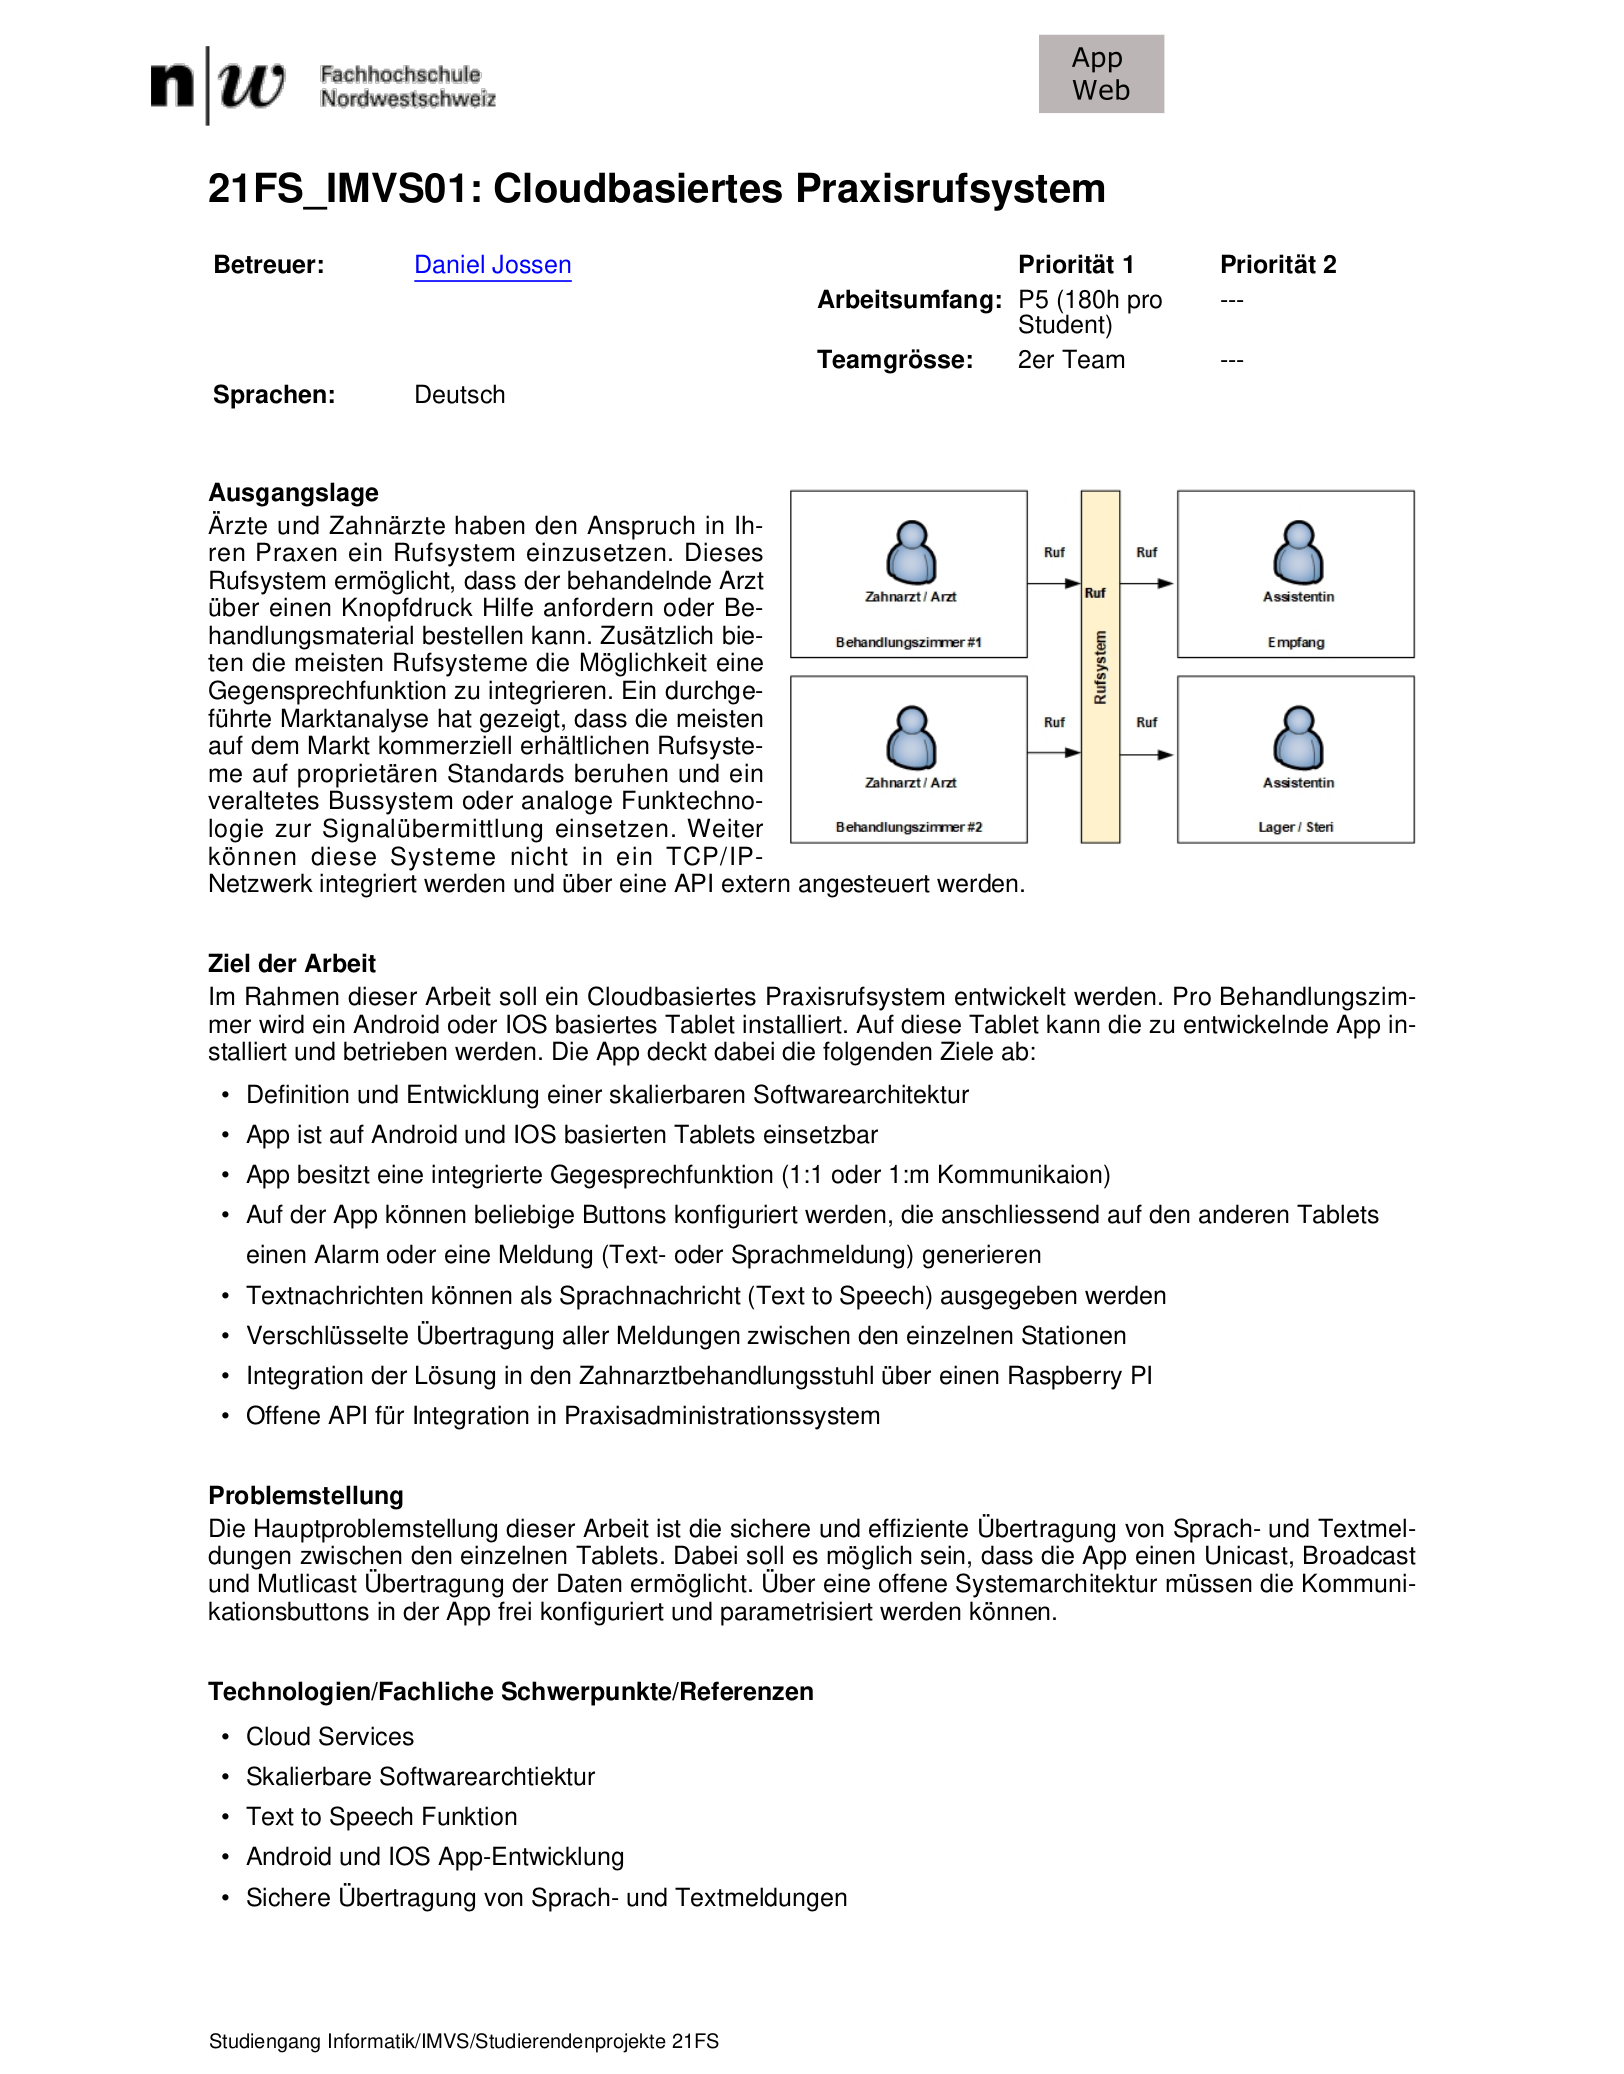
\includegraphics[width=\textwidth]{graphics/aufgabenstellung}
                \caption{Aufgabenstellung}
            \end{minipage}
        \end{figure}

    \clearpage
    \subsection{Quellcodeverwaltung}

    Sämtlicher Quellcode der im Rahmen des Projektes entsteht, wurde mit Git verwaltet. Der Quellcode ist für Berechtigte unter dem Projekt IP5-Cloudbasiertes-Praxisrufsystem auf github.com einsehbar.
    (Referenz https://github.com/IP5-Cloudbasiertes-Praxisrufsystem). Berechtigungen können bei Joshua Villing oder Kevin Zellweger angefordert werden.

    \begin{itemize}
        \item IP5-praxis-mobile-client
        \item IP5-praxis-cloud-service
        \item IP5-praxis-admin-ui
        \item IP5-praxis-documentation
    \end{itemize}

    \subsection{Benutzerhandbuch}

        \subsubsection*{Mobile Client}

        \textbf{Anmeldung und Konfiguration}

        \begin{enumerate}
            \item Mobile Client Applikation öffnen
            \item Gewünschte Konfiguration auswählen
        \end{enumerate}

        \textbf{Benachrichtigung empfangen}

        \begin{enumerate}
            \item In Mobile Client anmelden.
            \item In Navigationsleiste (unten) "Home" auswählen.
            \item Button mit dem gewünschten Titel antippen.
            \item Die Benachrichtigung wird automatisch versendet.
        \end{enumerate}

        \textbf{Benachrichtigung Auflisten und Quittieren}

        \begin{enumerate}
            \item In Mobile Client anmelden.
            \item In Navigationsleiste (unten) "Inbox" auswählen.
            \item In dieser Ansicht sehen Sie alle empfangenen noch nicht quittierten Benachrichtigungen.
            \item Zum Quittieren einer Benachrichtigung kann diese angetippt werden.
        \end{enumerate}

        \textbf{Abmeldung}

        \begin{enumerate}
            \item Mobile Client Applikation öffnen
            \item Auf den Namen in der Kopfleiste tippen
            \item Logout bestätigen
        \end{enumerate}



\subsubsection*{Admin UI}

    \subsection{Betriebshandbuch}
    \subsection{Entwicklerdokumentation}
    \subsection{Ehrlichkeitserklärung}
